
\section{Rules}
% \begin{figure}
%   \centering
%   
\includegraphics[width=0.9\columnwidth]{figures/sigchi-logo}
%   \caption{Insert a caption below each figure. Do not alter the
%     Caption style.  One-line captions should be centered; multi-line
%     should be justified. }~\label{fig:figure1}
% \end{figure}

% \begin{figure*}
%   \centering
%   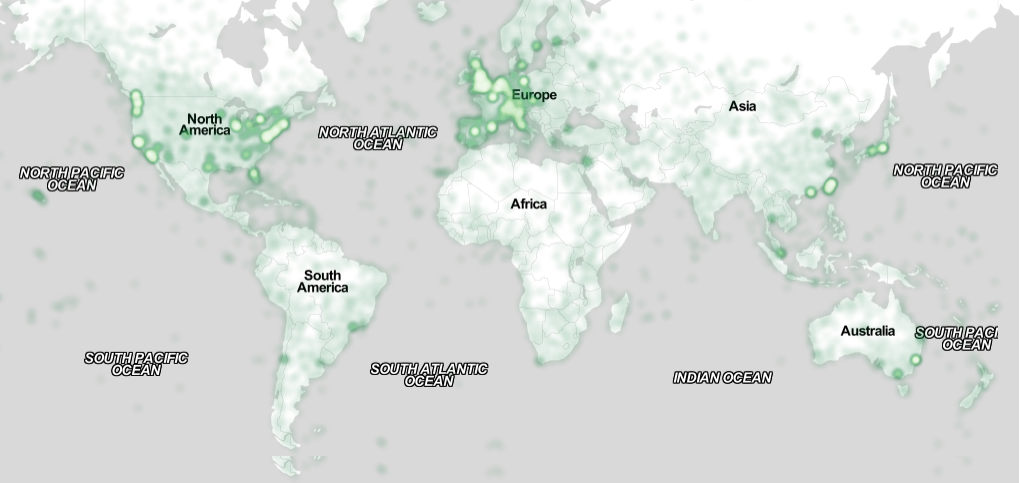
\includegraphics[width=1.75\columnwidth]{figures/map}
%   \caption{Figures as wide as you need, up to a maximum of the full width of
%     both columns. Note that \LaTeX\ tends to render large figures on a
%     dedicated page. Image: \ccbynd~ayman on
%     Flickr.}~\label{fig:figure2}
% \end{figure*}

% \begin{table}
%   \centering
%   \begin{tabular}{l r r r}
%     % \toprule
%     & & \multicolumn{2}{c}{\small{\textbf{Test Conditions}}} \\
%     \cmidrule(r){3-4}
%     {\small\textit{Name}}
%     & {\small \textit{First}}
%       & {\small \textit{Second}}
%     & {\small \textit{Final}} \\
%     \midrule
%     Marsden & 223.0 & 44 & 432,321 \\
%     Nass & 22.2 & 16 & 234,333 \\
%     Borriello & 22.9 & 11 & 93,123 \\
%     Karat & 34.9 & 2200 & 103,322 \\
%     % \bottomrule
%   \end{tabular}
%   \caption{Table captions should be placed below the table. We
%     recommend table lines be 1 point, 25\% black. Minimize use of
%     table grid lines.}~\label{tab:table1}
% \end{table}

% \begin{quote}
% Quotes like this
% \end{quote}
\begin{itemize}
	\item Include internet cites in references, and sometimes as URL in text
  \item Abstract: about 150 words
  \item Don't number sections
  \item Can use \texttt{{\textbackslash}section}, \texttt{{\textbackslash}subsection},
  and \texttt{{\textbackslash}subsubsection}
  \item For titles and headings, don't capitalize the or of unless they are the first word
  \item use Figure rather than fig
  \item Figures on top or bottom of columns
	\item Can have video if needed.
	\item use PDF or EPS for images
	\item Use \textit{``quotes inline like so''}
    \item PDFs must be ACM Compliant testing with Adobe Acrobat Reader v10
{\url{http://www.sheridanprinting.com/typedept/ACM-distilling-settings.htm}}
  \item Add alternative text to all figures
  \item Mark table headings
  \item Add tags to the PDF \url{http://chi2016.acm.org/accessibility}
  \item Verify the default language
  \item Set the tab order to ``Use Document Structure''
  \item Write in a straightforward style.
  \item Try to avoid long or complex sentence structures.
  \item Briefly define or explain all technical terms that may be
    unfamiliar to readers.
  \item Explain all acronyms the first time they are used in your
    text---e.g., ``Digital Signal Processing (DSP)''.
  \item Explain local references (e.g., not everyone knows all city
    names in a particular country).
  \item Explain ``insider'' comments. Ensure that your whole audience
    understands any reference whose meaning you do not describe (e.g.,
    do not assume that everyone has used a Macintosh or a particular
    application).
  \item Explain colloquial language and puns. Understanding phrases like
    ``red herring'' may require a local knowledge of English.  Humor and
    irony are difficult to translate.
  \item Use unambiguous forms for culturally localized concepts, such as
    times, dates, currencies, and numbers (e.g., ``1--5--97'' or
    ``5/1/97'' may mean 5 January or 1 May, and ``seven o'clock'' may
    mean 7:00 am or 19:00). For currencies, indicate equivalences:
    ``Participants were paid {\fontfamily{txr}\selectfont \textwon}
    25,000, or roughly US \$22.''
  \item Be careful with the use of gender-specific pronouns (he, she)
    and other gendered words (chairman, manpower, man-months). Use
    inclusive language that is gender-neutral (e.g., she or he, they,
    s/he, chair, staff, staff-hours, person-years). See the
    \textit{Guidelines for Bias-Free Writing} for further advice and
    examples regarding gender and other personal
    attributes~\cite{Schwartz:1995:GBF}. Be particularly aware of
    considerations around writing about people with disabilities.
  \item If possible, use the full (extended) alphabetic character set
    for names of persons, institutions, and places (e.g.,
    Gr{\o}nb{\ae}k, Lafreni\'ere, S\'anchez, Nguy{\~{\^{e}}}n,
    Universit{\"a}t, Wei{\ss}enbach, Z{\"u}llighoven, \r{A}rhus, etc.).
    These characters are already included in most versions and variants
    of Times, Helvetica, and Arial fonts.
\end{itemize}
